%package list
\documentclass{article}
\usepackage[top=3cm, bottom=3cm, outer=3cm, inner=3cm]{geometry}
\usepackage{multicol}
\usepackage{graphicx}
\usepackage{url}
%\usepackage{cite}
\usepackage{hyperref}
\usepackage{array}
%\usepackage{multicol}
\newcolumntype{x}[1]{>{\centering\arraybackslash\hspace{0pt}}p{#1}}
\usepackage{natbib}
\usepackage{pdfpages}
\usepackage{multirow}
\usepackage[normalem]{ulem}
\useunder{\uline}{\ul}{}
\usepackage{svg}
\usepackage{xcolor}
\usepackage{listings}
\lstdefinestyle{ascii-tree}{
    literate={├}{|}1 {─}{--}1 {└}{+}1 
  }
\lstset{basicstyle=\ttfamily,
  showstringspaces=false,
  commentstyle=\color{red},
  keywordstyle=\color{blue}
}
%\usepackage{booktabs}
\usepackage{caption}
\usepackage{subcaption}
\usepackage{float}
\usepackage{array}

\newcolumntype{M}[1]{>{\centering\arraybackslash}m{#1}}
\newcolumntype{N}{@{}m{0pt}@{}}


%%%%%%%%%%%%%%%%%%%%%%%%%%%%%%%%%%%%%%%%%%%%%%%%%%%%%%%%%%%%%%%%%%%%%%%%%%%%
%%%%%%%%%%%%%%%%%%%%%%%%%%%%%%%%%%%%%%%%%%%%%%%%%%%%%%%%%%%%%%%%%%%%%%%%%%%%
\newcommand{\itemEmail}{mvelasquea@unsa.edu.pe}
\newcommand{\itemStudent}{Mikhail Gabino Velasque Arcos}
\newcommand{\itemCourse}{Teoria FUNDAMENTOS DE LA PROGRAMACION II}
\newcommand{\itemCourseCode}{20214260}
\newcommand{\itemSemester}{II}
\newcommand{\itemUniversity}{Universidad Nacional de San Agustín de Arequipa}
\newcommand{\itemFaculty}{Facultad de Ingeniería de Producción y Servicios}
\newcommand{\itemDepartment}{Departamento Académico de Ingeniería de Sistemas e Informática}
\newcommand{\itemSchool}{Escuela Profesional de Ingeniería de Sistemas}
\newcommand{\itemAcademic}{2023 - B}
\newcommand{\itemInput}{Del  22 de diciembre 2023}
\newcommand{\itemOutput}{Al 23 de diciembre 2023}
\newcommand{\itemPracticeNumber}{03}
\newcommand{\itemTheme}{Resolucion de los problemas de teoria FP2}
%%%%%%%%%%%%%%%%%%%%%%%%%%%%%%%%%%%%%%%%%%%%%%%%%%%%%%%%%%%%%%%%%%%%%%%%%%%%
%%%%%%%%%%%%%%%%%%%%%%%%%%%%%%%%%%%%%%%%%%%%%%%%%%%%%%%%%%%%%%%%%%%%%%%%%%%%

\usepackage[english,spanish]{babel}
\usepackage[utf8]{inputenc}
\AtBeginDocument{\selectlanguage{spanish}}
\renewcommand{\figurename}{Figura}
\renewcommand{\refname}{Referencias}
\renewcommand{\tablename}{Tabla} %esto no funciona cuando se usa babel
\AtBeginDocument{%
	\renewcommand\tablename{Tabla}
}

\usepackage{fancyhdr}
\pagestyle{fancy}
\fancyhf{}
\setlength{\headheight}{30pt}
\renewcommand{\headrulewidth}{1pt}
\renewcommand{\footrulewidth}{1pt}
\fancyhead[L]{\raisebox{-0.2\height}{
\includegraphics[width=3cm]{img/logo_episunsa.png}}}
\fancyhead[C]{\fontsize{7}{7}\selectfont	\itemUniversity \\ \itemFaculty \\ \itemDepartment \\ \itemSchool \\ \textbf{\itemCourse}}
\fancyhead[R]{\raisebox{-0.2\height}{
\includegraphics[width=1.2cm]{img/logo_abet}}}
\fancyfoot[L]{Estudiante Mikhail Gabino Velasque Arcos}
\fancyfoot[C]{\itemCourse}
\fancyfoot[R]{Página \thepage}

% para el codigo fuente
\usepackage{listings}
\usepackage{color, colortbl}
\definecolor{dkgreen}{rgb}{0,0.6,0}
\definecolor{gray}{rgb}{0.5,0.5,0.5}
\definecolor{mauve}{rgb}{0.58,0,0.82}
\definecolor{codebackground}{rgb}{0.95, 0.95, 0.92}
\definecolor{tablebackground}{rgb}{0.8, 0, 0}

\lstset{frame=tb,
	language=bash,
	aboveskip=3mm,
	belowskip=3mm,
	showstringspaces=false,
	columns=flexible,
	basicstyle={\small\ttfamily},
	numbers=none,
	numberstyle=\tiny\color{gray},
	keywordstyle=\color{blue},
	commentstyle=\color{dkgreen},
	stringstyle=\color{mauve},
	breaklines=true,
	breakatwhitespace=true,
	tabsize=3,
	backgroundcolor= \color{codebackground},
}

\begin{document}
	
	\vspace*{10px}
	
	\begin{center}	
		\fontsize{17}{17} \textbf{ Informe de Ejercicios teoria 03 }
	\end{center}
	\centerline{\textbf{\Large Tema: Clases}}
	%\vspace*{0.5cm}	

	\begin{flushright}
		\begin{tabular}{|M{2.5cm}|N|}
			\hline 
			\rowcolor{tablebackground}
			\color{white} \textbf{Nota}  \\
			\hline 
			     \\[30pt]
			\hline 			
		\end{tabular}
	\end{flushright}	

	\begin{table}[H]
		\begin{tabular}{|x{4.7cm}|x{4.8cm}|x{4.8cm}|}
			\hline 
			\rowcolor{tablebackground}
			\color{white} \textbf{Estudiante} & \color{white}\textbf{Escuela}  & \color{white}\textbf{Asignatura}   \\
			\hline 
			{\itemStudent \par \itemEmail} & \itemSchool & {\itemCourse \par Semestre: \itemSemester \par Código: \itemCourseCode}     \\
			\hline 			
		\end{tabular}
	\end{table}		
	
	\begin{table}[H]
		\begin{tabular}{|x{4.7cm}|x{4.8cm}|x{4.8cm}|}
			\hline 
			\rowcolor{tablebackground}
			\color{white}\textbf{Laboratorio} & \color{white}\textbf{Tema}  & \color{white}\textbf{Duración}   \\
			\hline 
			\itemPracticeNumber & \itemTheme & 04 horas   \\
			\hline 
		\end{tabular}
	\end{table}
	
	\begin{table}[H]
		\begin{tabular}{|x{4.7cm}|x{4.8cm}|x{4.8cm}|}
			\hline 
			\rowcolor{tablebackground}
			\color{white}\textbf{Semestre académico} & \color{white}\textbf{Fecha de inicio}  & \color{white}\textbf{Fecha de entrega}   \\
			\hline 
			\itemAcademic & \itemInput &  \itemOutput  \\
			\hline 
		\end{tabular}
	\end{table}
%%%%%%%%%%%%%%%%%%%%%%%%%%%%%%%%%%%%%%%%%%%%%%%%%%%%%%%%%%%%%%%%%%%%%%%%%%%%
%%%%%%%%%%%%%%%%%%%%%%%%%%%%%%%%%%%%%%%%%%%%%%%%%%%%%%%%%%%%%%%%%%%%%%%%%%%%
	\section{Tarea}
	\begin{itemize}		
		\item Ejercicio 01: Crear una clase base denominada Puntoque conste de las coordenadas x e y. A 
partir de esta clase, definir una clase denominada Circulo que tenga las coordenadas del 
centro y un atributo denominado radio. Entre las funciones miembro de la primera clase, 
deberá existir una función distancia() que devuelva la distancia entre dos puntos, donde:
Distancia = ((x2 – x1)2 + (y2 – y1)2)1/2
		\item Ejercicio 02: Utilizando la clase construida en el ejercicio 01, obtener una clase derivada 
Cilindro derivada de Circulo. La clase Cilindro deberá tener una función miembro que calcule 
la superficie de dicho cilindro. La fórmula que calcula la superficie del cilindro es S = 2r(l + r) 
donde r es el radio del cilindro y l es la longitud.

		\item Caso de estudio especial: herencia múltiple. Es un tipo de herencia en la que una 
clase hereda el estado (estructura) y el comportamiento de más de una clase base. (hay 
herencia múltiple cuando una clase hereda de más de una clase). Java no permite la herencia 
múltiple, pero se puede conseguir la implementación de la herencia múltiple usando 
interfaces. Implemente el siguiente diagrama de clases UML y consiga pruebas válidas.
		\end{itemize}
	\section{Equipos, materiales y temas utilizados}
	\begin{itemize}
		\item Git , Git hub , clases, Diagramas UML ,herencia , herencia multiple
		\item VIM 9.0.
		\item OpenJDK 64-Bits 17.0.7.
		\item Git 2.39.2.
		\item Cuenta en GitHub con el correo institucional.
		\item Programación Orientada a Objetos.
	\end{itemize}
	
	\section{URL de Repositorio Github}
	\begin{itemize}
		\item URL del Repositorio GitHub para clonar o recuperar.
			\item URL :https://github.com/mvelasquea/fp2-23b.git

	\end{itemize}
	
	\section{Ejercicio 1:CREACION DE LAS CLASES PUNTO Y MAIN}
	
	\subsection{Creando la clase Punto/operaciones y la clase PRINCIPAL}
		
	\begin{lstlisting}[language=bash,caption={Creando la clase Punto}][H]
	
package problemas_ejercicio22_diciembre;
import java.util.*;
/*
	 Ejercicio de teoria ( ejercicio 1)
	 >	clase punto 
	 Autor :Mikhail Gabino Velasque Arcos
	colaboro:---
	tiempo:horas
	 */
//creaciond ela calse punto para acoplarlo a la clase pincipal llamada problema1_mains
public class Punto {
    int x, y;
    public Punto(int x, int y) {
        this.x = x;
        this.y = y;
    }
    //funcion que  aplica la forma de distancia entre puntos  haciendo el uso de math , pow(potencia), sqrt(raiz)
    // tomando los valores ya ingresados por el usuario 
    public double distancia(Punto otroPunto) {
        return Math.sqrt(Math.pow((otroPunto.x - this.x), 2) + Math.pow((otroPunto.y - this.y), 2));
    }
}	
	\end{lstlisting}
	\begin{lstlisting}[language=bash,caption={Creando la clase Main}][H]

package problemas_ejercicio22_diciembre;
import java.util.*;
/*
Ejercicio de teoria ( ejercicio 1)
>	clase PRINCIPAL MAIN 
Autor :Mikhail Gabino Velasque Arcos
colaboro:---
tiempo:horas
*/
public class problema1_main {
    public static void main(String[] args) {
        Scanner scanner = new Scanner(System.in);
// introduccion de valores tano del punto A como el del punto B 
        //Se obtiene  2 valores "x" y dos valores "y" respectivamente a los puntos ya antes mencionados
        System.out.println("Ingrese la coordenada x del primer punto: ");
        int x1 = scanner.nextInt();
        System.out.println("Ingrese la coordenada y del primer punto: ");
        int y1 = scanner.nextInt();

        Punto punto1 = new Punto(x1, y1);

        System.out.println("Ingrese la coordenada x del segundo punto: ");
        int x2 = scanner.nextInt();
        System.out.println("Ingrese la coordenada y del segundo punto: ");
        int y2 = scanner.nextInt();

        Punto punto2 = new Punto(x2, y2);
// se llama a la funcion de "distancia" para luego ejecutarla y mostrar el resultado
        System.out.println("La distancia entre los puntos es: " + punto1.distancia(punto2));
    }}

	\end{lstlisting}	
	
	\subsection{Resultados}
	
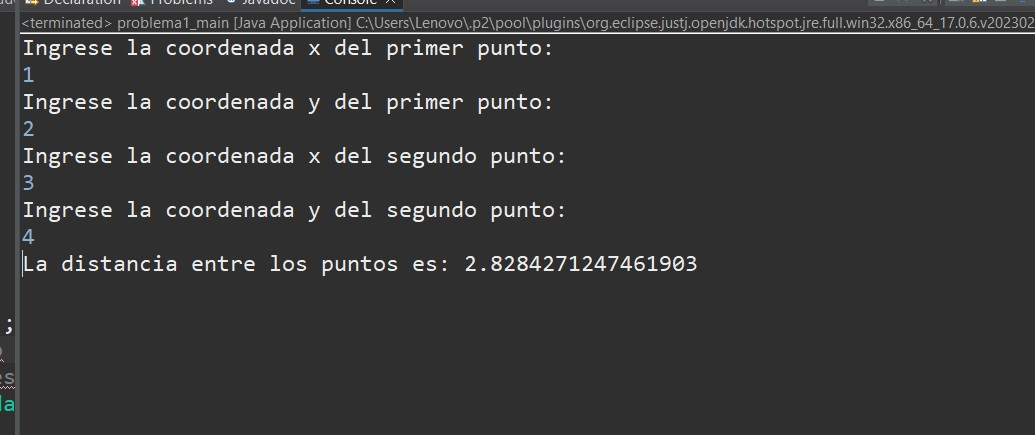
\includegraphics[scale=0.35]{img/captura1.jpeg} 	
	\begin{itemize}	
		\item Se muestra como el programa pide valores al usuario para completar el valor del punto 1 y del punto 2 para aplicar la funcion dentro de la clase punto (Dsitancia entre dos puntos)
	\end{itemize}
	
		\section{Ejercicio 2:CREACION DE LAS CLASES Cilindro Y Main}
	
	\subsection{Creando la clase Punto/operaciones y la clase PRINCIPAL}
		
	\begin{lstlisting}[language=bash,caption={Creando la clase cilindro}][H]
	package problemas_ejercicio22_diciembre;
/*Ejercicio de teoria ( ejercicio 2)
>	clase Cilindro 
Autor :Mikhail Gabino Velasque Arcos
colaboro:---
tiempo:horas
*/
// Clase derivada Cilindro de la clase Punto
public class Cilindro extends Punto {
    private double longitud; // Longitud del cilindro

    // Constructor que toma dos puntos y establece la longitud del cilindro
    public Cilindro(Punto punto1, Punto punto2, double longitud) {
        super(punto1.x, punto1.y); // Llama al constructor de la clase base (Punto) para establecer las coordenadas del punto
        this.longitud = longitud;
    }
   // Función para calcular la superficie del cilindro
    public double calcularSuperficie() {
        double radio = distancia(new Punto(0, 0)); // Usa la distancia entre el punto y el origen como el radio
        return 2 * Math.PI * radio * (longitud + radio);
    }
}}
	\end{lstlisting}
	\begin{lstlisting}[language=bash,caption={Creando la clase Main}][H]


import java.util.Scanner;
/*Ejercicio de teoria ( ejercicio 2)
>	clase main  
Autor :Mikhail Gabino Velasque Arcos
colaboro:---
tiempo:horas
*/
public class problema2_main {
    public static void main(String[] args) {
        Scanner scanner = new Scanner(System.in);

        //solicitando valores de los puntos al usuario  al igual que la longitud 
        System.out.println("Ingrese la coordenada x del primer punto: ");
        int x1 = scanner.nextInt();
        System.out.println("Ingrese la coordenada y del primer punto: ");
        int y1 = scanner.nextInt();

        Punto punto1 = new Punto(x1, y1);

        System.out.println("Ingrese la coordenada x del segundo punto: ");
        int x2 = scanner.nextInt();
        System.out.println("Ingrese la coordenada y del segundo punto: ");
        int y2 = scanner.nextInt();

        Punto punto2 = new Punto(x2, y2);

        System.out.println("Ingrese la longitud del cilindro: ");
        double longitudCilindro = scanner.nextDouble();

        // creando el objeto de cilindro
        Cilindro cilindro = new Cilindro(punto1, punto2, longitudCilindro);

        // manda valores a la clase cilindro y lo calcula para mostrarlo
        System.out.println("La superficie del cilindro es: " + cilindro.calcularSuperficie());
    }
}


	\end{lstlisting}	
	
	\subsection{Resultados}
	
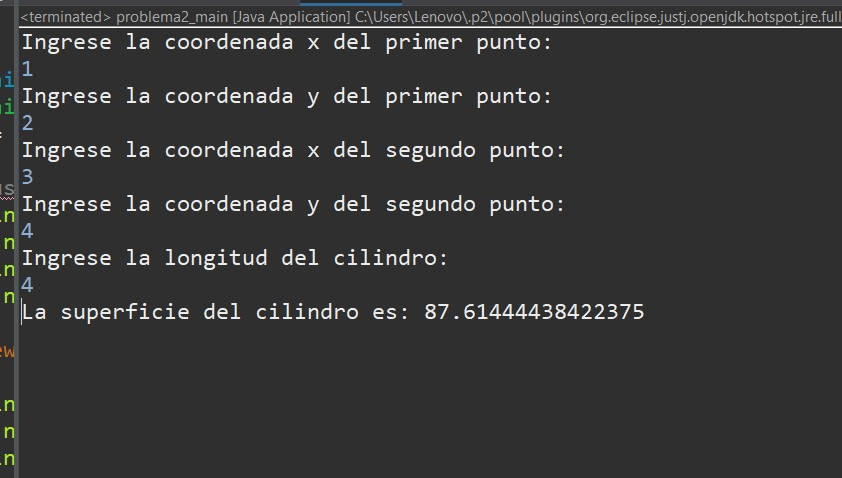
\includegraphics[scale=0.35]{img/captura2.jpeg} 
		\item Se muestra que con ayuda del codigo del anterior ejercicio usa el valor ya encontrado (radio) o la distandia entre 1 punto all otro ,  aplica la formula ya dada y ejecuta mostrando el resulto
	
	\end{itemize}
	
\begin{lstlisting}[style=ascii-tree]
teoria/
|--- Ejercicio1.java
|--- Ejercicio2.java
|--- Ejercicio3.java
|--- gitignore.java

|--- latex
    |--- img
    |   |--- logo_abet.png
    |   |--- logo_episunsa.png
    |   |--- logo_unsa.jpg
    |   |--- captura1.png    
    |   |--- captura2.png    

    |--- latex_ejercicio3_teoria_fp2.0.pdf    
    |--- latex_ejercicio3_teoria_fp2.0.tex
    |--- src
        |--- ejercicio1.java
        |--- ejercicio2.java
        |--- ejercicio3.java
\end{lstlisting}    

\section{Ejercicio 3:CREACION DE una clase UML  }
	
	\subsection{Creando un diagrama UML donde se usa una herencia multiple   con el grafico ya mostrado}
		
	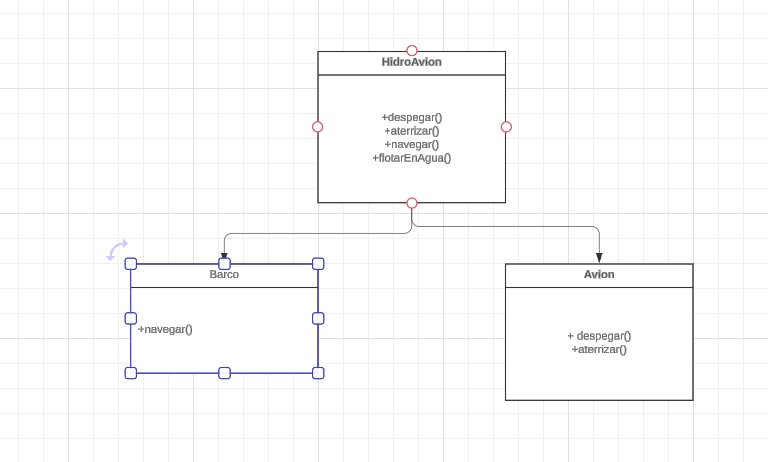
\includegraphics[scale=0.5]{img/captura3.jpeg} 
	
	
	
%\clearpage
%\bibliographystyle{apalike}
%\bibliographystyle{IEEEtranN}
%\bibliography{bibliography}
			
\end{document}